\section{Подходы к написанию автоматизированных тестов} 

Процесс тестирования прогараммного обеспечения можно разделить на две фазы: разработка тестовых сценариев и запуск тестовых сценариев. 

Разработка тестовых сценариев подразуевает анализ, дизайн и написание кода. Смысл этой фазы состоит в том, что бы разработать такое множество тестовых сценариев, которое бы удовлетворяло стандартам качества разрабатываемого программного обеспечения. Понятие <<автоматизированное тестирование>> не включает в себя автоматизацию этой фазы.

Вторая фаза подразумевает инсталяцию программного обеспечения и выполнение тестовых сценариев, разработанных на первой фазе. Запуск тестовых сценариев чаще всего автоматизируется. 


Разработка тестовых сценариев~--- комплексная задача. Сложность ее состоит в нахождении достаточного набора тестовых сценариев, который удовлетворяет стандартам качества. Одновременно с этим, набор тестов должен быть конечен и выполняться достаточно быстро. Далее будут рассмотренны техники анализа, дизайна и написания тестовых сценариев.


\subsection{Тестирование на основе спецификации} 

Спецификация~--- набор требований к программному обеспечению. Может быть представлена как текстовый файл или UML диаграмма.

Тестирование на основе спецификации~--- подход к разработке минимального набора тестов, которые будут удовлетворять спецификации. Такой подход позволяет абстрагироваться от конкретной реализации системы (тестирование <<черного ящика>>).

Основу этого метода составляет группировка множества входных данных.

\subsubsection{Группировка множества входных данных}

Пример спецификации. Определение високосного года. На вход программе поступает год в виде числа, программа должна возвращать \texttt{true} если год явлется висококосным и \texttt{false} в противном случае. Год високосный, если:

\begin{itemize}
	\item год кратен 4;
	\item год не кратен 100;
	\item исключение: если год кратен 400, то он високосный.
\end{itemize}

Реализация спецификации представленна в листинге 1.3.

\begin{ListingEnv}[!h]% настройки floating аналогичны окружению figure
	\captiondelim{ } % разделитель идентификатора с номером от наименования
	\caption{Определение високосного года}
	% окружение учитывает пробелы и табуляции и применяет их в сответсвии с настройками
	\begin{lstlisting}[language={Java}]
public class LeapYear {
	
	public boolean isLeapYear(int year) {
		if (year % 400 == 0)
		return true;
		if (year % 100 == 0)
		return false;
		
		return year % 4 == 0;
	}
}
	\end{lstlisting}
\end{ListingEnv}%

 Для подбора оптимальных входных данных, нужно разбить программу на классы(группы). Другими словами, нужно разбить множество входных данных следующим образом:
 
 \begin{enumerate}
 	\item каждый класс уникален, т.~е. не существует двух классов, которые приводят к одному и тому же поведению программы;
 	\item поведение программы может быть однозначно интерптитированно как корректное или не корректное.
 \end{enumerate}

Учитывая требования к классам и спецификацию, можно получить следующий набор классов:

 \begin{itemize}
 	\item год кратен 4, но не кратен 100~--- високосный, \texttt{true};
 	\item год кратен 4, кратен 100, кратен 400~--- високосный, \texttt{true};
 	\item год не кратен 4~--- не високосный, \texttt{false};
 	\item год кратен 4, кратен 100, но не кратен 400~--- не високосный, \texttt{false}.
 \end{itemize}

Каждый класс может быть выражен в бесконечном множестве входных данных. Однако, каждый конкретный набор входных данных из одного и того же класса, провоцирует одно и то же поведение программы. Таким образом классы образуют классы эквивалентности. Достаточно выбрать один набор входных данных из каждого класса:

 \begin{itemize}
	\item 2016, год кратен 4, но не кратен 100;
	\item 2000, год кратен 4, кратен 100, кратен 400;
	\item 39, год не кратен 4;
	\item 1900, год кратен 4, кратен 100, но не кратен 400.
\end{itemize}

Пример тестирующего кода представлен в листинге~1.4.

\begin{ListingEnv}[!h]% настройки floating аналогичны окружению figure
	\captiondelim{ } % разделитель идентификатора с номером от наименования
	\caption{Теструющий класс \textit{LeapYearTest}}
	% окружение учитывает пробелы и табуляции и применяет их в сответсвии с настройками
	\begin{lstlisting}[language={Java}]
public class LeapYearTest {
	
	private final LeapYear leapYear = new LeapYear();
	
	@Test
	public void divisibleBy4_notDivisibleBy100() {
		boolean leap = leapYear.isLeapYear(2016);
		assertTrue(leap);
	}
	
	@Test
	public void divisibleBy4_100_400() {
		boolean leap = leapYear.isLeapYear(2000);
		assertTrue(leap);
	}
	
	@Test
	public void notDivisibleBy4() {
		boolean leap = leapYear.isLeapYear(39);
		assertFalse(leap);
	}
	
	@Test
	public void divisibleBy4_and_100_not_400() {
		boolean leap = leapYear.isLeapYear(1900);
		assertFalse(leap);
	}
}
	\end{lstlisting}
\end{ListingEnv}%



\subsection{Тестирование границ} 
 
Ошибки, основанные на граничных условиях очень распростаннены. Например, разработчики часто ошибаются в операторах <<больше>> (\texttt{>}) или <<больше или равно>> (\texttt{>=}). Техника тестирования границ позволяет избежать подобных ошибок.

\subsubsection{Границы между классами} 

В предыдущем разделе описан подход к написанию тестов с помощью классов эквивалентности. Эти классы имеют границы. Другими словами, если применять маленькие изменения к входным данным (например, +1) рано или поздно набор входных данных перейдет в другой класс. Конкретная точка, в которой входные данные переходят из одного класса в другой, называется \textit{граничным значением}. Суть тестирования границ~--- тестирование корректности программы на граничных значениях. 

Более формально, граничные значения~--- это два набора ближайших к друг другу входных данных \([p_1, p_2]\), где \(p_1\) относится к группе \(A\), а \(p_2\) относится к групе \(B\).
 
На практике тестирование границ комбинируется с тестированием, основанным на спецификации. Такая комбинация называется \textit{доменным тестированием}.
 
\subsubsection{Пример тестирования границ} 

Постановка задачи. Подсчет количества очков игрока. Даны очки игрока и количество оставшихся жизней, программа должна:

\begin{itemize}
	\item Если количество очков игрока меньше 50, то всегда добавлять 50 очков к текущему значению.
	\item Если количество очков игрока больше или равно 50, то:
	\begin{itemize}
		\item Если количество оставшихся жизней больше, чем 3, то умножить очки игрока на 3.
		\item Иначе добавить 30 очков к текущему значению.
	\end{itemize}
\end{itemize}

Реализация поставленной задачи представлена в листинге~1.5.

\begin{ListingEnv}[!h]% настройки floating аналогичны окружению figure
	\captiondelim{ } % разделитель идентификатора с номером от наименования
	\caption{Подсчет количества очков игрока}
	% окружение учитывает пробелы и табуляции и применяет их в сответсвии с настройками
	\begin{lstlisting}[language={Java}]
public class PlayerPoints {
	
	public int totalPoints(int currentPoints, int remainingLives) {
		if(currentPoints < 50)
		return currentPoints+50;
		
		return remainingLives < 3 ? currentPoints+30 : currentPoints*3;
	}
}
	\end{lstlisting}
\end{ListingEnv}%

Разбитие входных данных на классы выглядит следующим образом:

\begin{enumerate}
	\item Количество очков < 50.
	\item Количество очков >= 50 и оставшихся жизней < 3.
	\item Количество очков >= 50 и оставшихся жизней >= 3.
\end{enumerate}

Тестирующий код представлен в листинге~1.6.

\begin{ListingEnv}[!h]% настройки floating аналогичны окружению figure
	\captiondelim{ } % разделитель идентификатора с номером от наименования
	\caption{Тестирующий код}
	% окружение учитывает пробелы и табуляции и применяет их в сответсвии с настройками
	\begin{lstlisting}[language={Java}]
public class PlayerPointsTest {
	
	private final PlayerPoints pp = new PlayerPoints();
	
	@Test
	void lessPoints() {
		assertEquals(30+50, pp.totalPoints(30, 5));
	}
	
	@Test
	void manyPointsButLittleLives() {
		assertEquals(300+30, pp.totalPoints(300, 1));
	}
	
	@Test
	void manyPointsAndManyLives() {
		assertEquals(500*3, pp.totalPoints(500, 10));
	}
}
	\end{lstlisting}
\end{ListingEnv}%

Определение граничных значений: 

\begin{enumerate}
	\item \textbf{Граничное значение 1:} Когда количество очков строго меньше, чем 50, набор входных данных относится к группе 1. Если количество очков больше или равно 50, набор входных данных относится к группам 2 и 3. Таким образом, граничные значения равны 49 и 50.
	\item \textbf{Граничное значение 2:}  Когда количество очков больше или равно 50 и количество оставшихся жизней меньше6 чем 3, тогда набор данных относится к группе 2, иначе он относится к группе 3.

Получившиеся границы представленны на рис.~1.1.

\begin{figure}[ht]
	\centering
	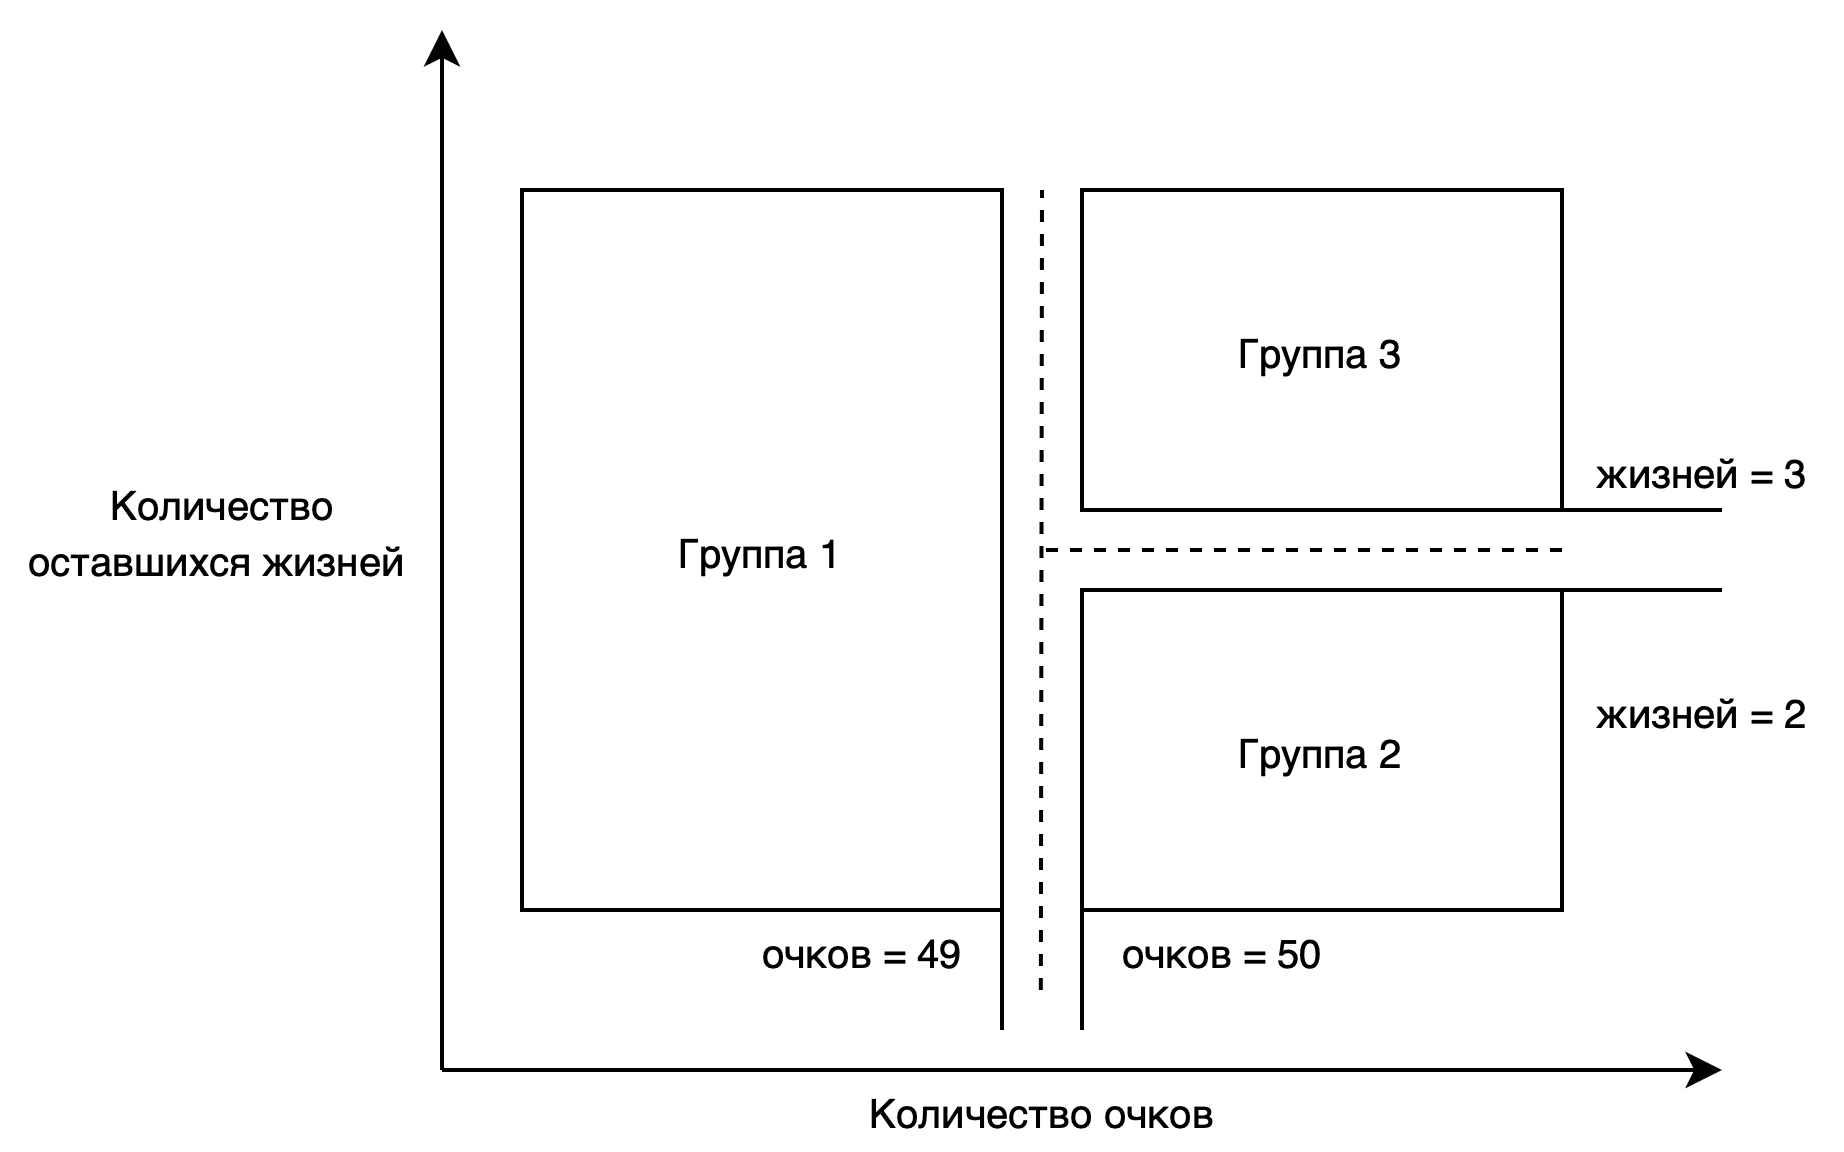
\includegraphics [scale=1] {Boundaries_example}
	\caption{Границы групп}
	\label{img:Boundaries_example}
\end{figure}

Тестирующий код представлен в листинге~1.7.

\begin{ListingEnv}[!h]% настройки floating аналогичны окружению figure
	\captiondelim{ } % разделитель идентификатора с номером от наименования
	\caption{Тестирование границ}
	% окружение учитывает пробелы и табуляции и применяет их в сответсвии с настройками
	\begin{lstlisting}[language={Java}]
@Test
void betweenLessAndManyPoints() {
	assertEquals(49+50, pp.totalPoints(49, 5));
	assertEquals(50*3, pp.totalPoints(50, 5));
}

@Test
void betweenLessAndManyLives() {
	assertEquals(500*3, pp.totalPoints(500, 3));
	assertEquals(500+30, pp.totalPoints(500, 2));
}
	\end{lstlisting}
\end{ListingEnv}%



\subsection{Структурное тестирование} 
 
 \fixme{TBD}
 

\subsection{Тестирование на основе модели} 
 
 \fixme{TBD}
 

\subsection{Тестирование на основе контракта} 
 
 \fixme{TBD}


\subsection{Тестирование свойств} 

\fixme{TBD}